%--------------------------------------------------------
% TEMPLATE PARA TRABALHO DE GRADUAÇÃO
% Universidade Estadual Paulista ``Júlio de Mesquita Filho'' - UNESP - ICT - São José dos Campos
% Engenharia Ambiental
%
% Customização da classe abnTeX2 (http://www.abntex.net.br/) para as normas da UNESP - ICT
%
% Autor: Luccas Zambon Maselli (v.1 -- 03jun2019)
%		 Rogério Galante Negri (v.2 -- 22mai2022)
%
%--------------------------------------------------------
% Codificação: UTF-8
% LaTeX:  abnTeX2          
% -------------------------------------------------------


% CARREGA CLASSE PERSONALIZADA---------------------------
\documentclass[%twoside, % Impressão em frente e verso
			   openany,
    	       oneside,  % Impressão apenas frente
]{configuracoes/utfpr-abntex2}


% INCLUI ARQUIVOS DE CONFIGURAÇÕES-----------------------
% REFERÊNCIAS------------------------------------------------------------------
\usepackage[%
    alf,
    abnt-emphasize=bf,
    bibjustif,
    recuo=0cm,
    abnt-url-package=url,       % Utiliza o pacote url
    abnt-refinfo=yes,           % Utiliza o estilo bibliográfico abnt-refinfo
    abnt-etal-cite=3,
    abnt-etal-list=3,
    abnt-thesis-year=final
]{abntex2cite}                  % Configura as citações bibliográficas conforme a norma ABNT

% PACOTES----------------------------------------------------------------------
\usepackage{ae, aecompl}                                    % Fontes de alta qualidade
\usepackage{amsfonts, amssymb, amsmath}                     % Fontes e símbolos matemáticos
\usepackage[algoruled, portuguese]{algorithm2e}             % Permite escrever algoritmos em português
\usepackage{booktabs}                                       % Réguas horizontais em tabelas
\usepackage{caption, subcaption}
\usepackage{color, colortbl}                                % Controle das cores
\usepackage{caption}
\usepackage[labelfont=bf]{caption}													% Caption em negrito
\usepackage{float}                                          % Necessário para tabelas/figuras em ambiente multi-colunas
\usepackage[T1]{fontenc}                                    % Seleção de código de fonte
\usepackage[bottom]{footmisc}                               % Mantém as notas de rodapé sempre na mesma posição

%\usepackage[a4paper,left=3cm,right=2cm,top=3cm,bottom=2cm]{geometry}
\usepackage{geometry}
\geometry{a4paper,total={210mm,297mm},left=20mm,right=20mm,top=30mm,bottom=20mm}

\usepackage{graphicx}                                       % Inclusão de gráficos e figuras
\usepackage{icomma}                                         % Uso de vírgulas em expressões matemáticas
\usepackage{indentfirst}                                    % Indenta o primeiro parágrafo de cada seção
\usepackage[utf8]{inputenc}                                 % Codificação do documento
\usepackage{latexsym}                                       % Símbolos matemáticos
\usepackage{lscape}                                         % Permite páginas em modo "paisagem"
\usepackage{lastpage}                                       % Para encontrar última página do documento
\usepackage{lipsum}
\usepackage{listings}
\usepackage{listingsutf8}
\usepackage{microtype}                                      % Melhora a justificação do documento
\usepackage{multirow, array}                                % Permite tabelas com múltiplas linhas e colunas
\usepackage{pdfpages}
\usepackage{subeqnarray}                                    % Permite subnumeração de equações
\usepackage{siunitx}
\usepackage[figtopcap]{subfigure} 
\usepackage{times}                                          % Usa a fonte Times
\usepackage{verbatim}                                       % Permite apresentar texto tal como escrito no documento, ainda que sejam comandos Latex
\usepackage[table,xcdraw]{xcolor}
%\usepackage[scaled]{helvet}                               % Usa a fonte Helvetica
%\usepackage{uarial}
%\usepackage{palatino}                                      % Usa a fonte Palatino
%\usepackage{lmodern}                                       % Usa a fonte Latin Modern
%\usepackage{picinpar}                                      % Dispor imagens em parágrafos
%\usepackage{scalefnt}                                      % Permite redimensionar tamanho da fonte
%\usepackage{subfig}                                        % Posicionamento de figuras
%\usepackage{upgreek}                                       % Fonte letras gregas

\usepackage{tabularx}


\newcolumntype{L}[1]{>{\raggedright\let\newline\\\arraybackslash\hspace{0pt}}m{#1}}
\newcolumntype{C}[1]{>{\centering\let\newline\\\arraybackslash\hspace{0pt}}m{#1}}
\newcolumntype{R}[1]{>{\raggedleft\let\newline\\\arraybackslash\hspace{0pt}}m{#1}}


\usepackage[format=hang,font=normalsize,labelfont=nf]{caption}  %<--- Tipo do ambiente em tamanho normal e sem negrito/itálico


%\newcommand*{\noaddvspace}{\renewcommand*{\addvspace}[1]{}}
%\addtocontents{lof}{\protect\noaddvspace}
%\addtocontents{lof}{\linespread{1.5cm}}


% CONFIGURAÇÕES DE APARÊNCIA DO PDF FINAL--------------------------------------
\makeatletter
\hypersetup{%
    portuguese,
    colorlinks=false%true,   % true: "links" coloridos; false: "links" em caixas de texto
    linkcolor=blue,    % Define cor dos "links" internos
    citecolor=blue,    % Define cor dos "links" para as referências bibliográficas
    filecolor=blue,    % Define cor dos "links" para arquivos
    urlcolor=blue,     % Define a cor dos "hiperlinks"
    breaklinks=true,
    pdftitle={\@title},
    pdfauthor={\@author},
    pdfkeywords={abnt, latex, abntex, abntex2}
}
\makeatother

% ALTERA O ASPECTO DA COR AZUL--------------------------------------------------
\definecolor{blue}{RGB}{41,5,195}

% REDEFINIÇÃO DE LABELS---------------------------------------------------------
\renewcommand{\algorithmautorefname}{Algoritmo}
\def\equationautorefname~#1\null{Equa\c c\~ao~(#1)\null}

% CRIA ÍNDICE REMISSIVO---------------------------------------------------------
\makeindex

% HIFENIZAÇÃO DE PALAVRAS QUE NÃO ESTÃO NO DICIONÁRIO---------------------------
\hyphenation{%
    qua-dros-cha-ve
    Kat-sa-gge-los
}





\makeatletter
\providecommand\phantomcaption{\caption@refstepcounter\@captype}
\makeatother


% INCLUI ARQUIVOS DO TRABALHO (PRÉ-TEXTUAIS, TEXTUAIS, PÓS-TEXTUAIS)

% INSERE CAPA E FOLHA DE ROSTO
% CAPA---------------------------------------------------------------------------------------------------

% ORIENTAÇÕES GERAIS-------------------------------------------------------------------------------------
% Caso algum dos campos não se aplique ao seu trabalho, como por exemplo,
% se não houve coorientador, apenas deixe vazio.
% Exemplos: 
% \coorientador{}
% \departamento{}

% DADOS DO TRABALHO--------------------------------------------------------------------------------------
%\titulo{\MakeUppercase{Título do Trabalho}}
%\titulo{\MakeUppercase{Título do Trabalho}: subtítulo se houver}
\titulo{Título do Trabalho}
\subtitulo{subtítulo se houver} %<--- em revisão!

\titleabstract{English title}
\subtitle{subtitle}

\autor{\textbf{\uppercase{Nome do Aluno}}}  %É convertido automaticamente para maiúsculo/negrito
\autorcitacao{SOBRENOME, Nome do autor} % Sobrenome em maiúsculo e iniciais do nome e demais sobrenomes
\local{São José dos Campos}
\data{Ano de defesa}

% NATUREZA DO TRABALHO-----------------------------------------------------------------------------------
% Opções: 
% - Trabalho de Conclusão de Curso (se for Graduação)
% - Dissertação (se for Mestrado)
% - Tese (se for Doutorado)
% - Projeto de Qualificação (se for Mestrado ou Doutorado)
\projeto{Trabalho de graduação}

% TÍTULO ACADÊMICO---------------------------------------------------------------------------------------
% Opções:
% - Bacharel ou Tecnólogo (Se a natureza for Trabalho de Conclusão de Curso)
% - Mestre (Se a natureza for Dissertação)
% - Doutor (Se a natureza for Tese)
% - Mestre ou Doutor (Se a natureza for Projeto de Qualificação)
\tituloAcademico{Bacharel}

% ÁREA DE CONCENTRAÇÃO E LINHA DE PESQUISA---------------------------------------------------------------
% Se a natureza for Trabalho de Conclusão de Curso, deixe ambos os campos vazios
% Se for programa de Pós-graduação, indique a área de concentração e a linha de pesquisa
\areaconcentracao{}
\linhapesquisa{}

% DADOS DA INSTITUIÇÃO-----------------------------------------------------------------------------------
% Se a natureza for Trabalho de Conclusão de Curso, coloque o nome do curso de graduação em "programa"
% Formato para o logo da Instituição: \logoinstituicao{<escala>}{<caminho/nome do arquivo>}
\instituicao{Universidade Estadual Paulista ``Júlio de Mesquita Filho'' -- Unesp}
\departamento{Departamento de Engenharia Ambiental}
\programa{Engenharia Ambiental}

\instituicaoCurto{Universidade Estadual Paulista (Unesp)}
\instituicaoCampus{Instituto de Ciência e Tecnologia}


\tituloAcademicoEn{Degree}
\programaEn{Environmental Engineering}
\instituicaoCurtoEn{São Paulo State University (Unesp)}
\instituicaoCampusEn{Institute of Science and Technology}



%\logoinstituicao{0.2}{dados/figuras/logo-instituicao.png} 

% DADOS DOS ORIENTADORES---------------------------------------------------------------------------------
\orientador{Título e nome do orientador}
%\orientador[Orientadora:]{Nome da orientadora}
\instOrientador{Instituição do Orientador} % Universidade Estadual Paulista ``Júlio de Mesquita Filho'' caso pertencer ao departamento

\coorientador{}
%\coorientador[Coorientadora:]{Nome da coorientadora}
\instCoorientador{}

% FOLHA DE ROSTO--------------------------------------------------------------------------------------------------------

% TRABALHO DE CONCLUSÃO DE CURSO
 \preambulo{{\imprimirprojeto} apresentado como requisito parcial para a obtenção do título de {\imprimirtituloAcademico} em {\imprimirprograma} pela {\imprimirinstituicao}.}

% DISSERTAÇÃO DE MESTRADO
% \preambulo{{\imprimirprojeto} apresentada ao Programa de \mbox{Pós-graduação} da {\imprimirinstituicao}, como requisito parcial para obtenção do título de {\imprimirtituloAcademico}.}

% TESE DE DOUTORADO
% \preambulo{{\imprimirprojeto} apresentada ao Programa de \mbox{Pós-graduação} da {\imprimirinstituicao}, como requisito parcial para a obtenção do título de {\imprimirtituloAcademico}.}

% PROJETO DE QUALIFICAÇÃO DE MESTRADO OU DOUTORADO
%\preambulo{{\imprimirprojeto} apresentado ao Programa de \mbox{Pós-graduação} da {\imprimirinstituicao}, como requisito parcial para a obtenção do título de {\imprimirtituloAcademico}.}

% OBSERVAÇÕES-----------------------------------------------------------------------------------------------------------
% Altere este arquivo APENAS comentando as linhas que não se aplicam ao tipo de trabalho acadêmico desejado.



\begin{document}

\pretextual
\imprimircapa             % Comando para imprimir Capa
\imprimirfolhaderosto{}   % Comando para imprimir Folha de rosto

% INSERE ELEMENTOS PRÉ-TEXTUAIS
% -----------------------------------------------------------------------------
% Folha de Aprovação
% -----------------------------------------------------------------------------
%
%\textopadraofolhadeaprovacao{Esta folha deverá ser substituída pela cópia digitalizada da folha de aprovação fornecida.}

% -----------------------------------------------------------------------------
% Este documento foi mantido apenas para preservar a paginação do trabalho
% acadêmico final, após a inserção da folha de aprovação fornecida
% -----------------------------------------------------------------------------

\begin{folhadeaprovacao}[FOLHA DE APROVAÇÃO]
%\includepdf{folha_aprovacao_ass.pdf} Adicionar o pdf da folha assinada após aprovação

% MODELO DA FOLHA DE APROVAÇÃO
\begin{center}
{\large{\textbf{BANCA EXAMINADORA}}}

\vspace{3.5cm}


\begin{normalsize}

\rule{12cm}{1pt} \\
\textbf{Título e nome do orientador} \\
Universidade \\
Faculdade ou Instituto \\
Departamento \\

\vspace{4cm}

\rule{12cm}{1pt} \\
\textbf{Título e nome do avaliador} \\
Universidade \\
Faculdade ou Instituto \\
Departamento \\

\vspace{4cm}

\rule{12cm}{1pt} \\
\textbf{Título e nome do avaliador} \\
Universidade \\
Faculdade ou Instituto \\
Departamento \\

\end{normalsize}

\end{center}  

\vspace{2cm}

\begin{flushright}
São José dos Campos, data da apresentação.
\end{flushright}
  
\end{folhadeaprovacao}
   % Folha de aprovaćão


%\renewcommand{\dedicatorianame}{DEDICATÓRIA}
%
%\begin{dedicatoria}
%
%Inserir dedicatória do seu trabalho.
%
%\end{dedicatoria}


% DEDICATÓRIA------------------------------------------------------------------
%Mesmo ambiente dos "agradecimentos"

\begin{agradecimentos}[\large{DEDICATÓRIA}] 

\begin{center}
\vspace{-1cm}
\textcolor{blue}{OPCIONAL}
\end{center}

%Escreva sua dedicatória aqui, mas antes remova/comente o comando "\lipsum[1-2]"
\lipsum[3]


\end{agradecimentos}       % Dedicatória
% AGRADECIMENTOS---------------------------------------------------------------

\begin{agradecimentos}[\large{AGRADECIMENTOS}]

\begin{center}
\vspace{-1cm}
\textcolor{blue}{OPCIONAL}
\end{center}

%Escreva seus agradecimentos aqui, mas antes remova/comente o comando "\lipsum[1-2]"
\lipsum[1-2]


\end{agradecimentos}    % Agradecimentos
% EPÍGRAFE---------------------------------------------------------------------

\renewcommand{\epigraphname}{EPÍGRAFE}

\begin{epigrafe}

\begin{flushright}
\textit{
``Feliz aquele que transfere o que sabe e aprende o que ensina.'' \\ Cora Coralina, em Vintém de Cobre
}

\textcolor{blue}{OPCIONAL}
\end{flushright}

\end{epigrafe}

% OBSERVAÇÕES------------------------------------------------------------------
% Altere o texto para inserir a epígrafe do seu trabalho

          % Epígrafe

% RESUMO--------------------------------------------------------------------------------
% Não altere esta seção do texto--------------------------------------------------------
\newpage
%\phantomsection
%\addcontentsline{toc}{chapter}{RESUMO}
\begin{Spacing}{1}

\begin{resumo}[RESUMO]

%---------------------------------------------------------------------------------------
\noindent
{\imprimirautorcitacao}. 
   \ifx\imprimirtitulo\empty   
      \textbf{\imprimirtitulo}.
   \else
      \textbf{{\imprimirtitulo}: }{\imprimirsubtitulo}.
   \fi
{\imprimirdata}. {\imprimirprojeto} ({\imprimirtituloAcademico} em {\imprimirprograma}) -- {\imprimirInstituicaoCurto}, {\imprimirInstituicaoCampus}, {\imprimirlocal}, {\imprimirdata}.

\vspace{1cm}
%---------------------------------------------------------------------------------------



%O Resumo é um elemento obrigatório do TG. Fornece uma visão rápida e clara do conteúdo do estudo. O resumo deve ser redigido em parágrafo único, espaçamento simples e seguido das palavras representativas do conteúdo do estudo, as palavras-chave.

\lipsum[10] \lipsum[11] \lipsum[12] \lipsum[13]

\vspace{1cm}
Palavras-chave: assunto; assunto; assunto; assunto; assunto.
 
\end{resumo}

% OBSERVAÇÕES---------------------------------------------------------------------------
% Altere o texto inserindo o Resumo do seu trabalho.
% Escolha de 3 a 5 palavras ou termos que descrevam bem o seu trabalho 

\end{Spacing}







%
%% RESUMO--------------------------------------------------------------------------------
%
%\begin{resumo}[RESUMO]
%\begin{SingleSpacing}
%
%% Não altere esta seção do texto--------------------------------------------------------
%%\imprimirautorcitacao. \imprimirtitulo. \imprimirdata. \pageref {LastPage} f. \imprimirprojeto\ – \imprimirprograma, \imprimirinstituicao. \imprimirlocal, \imprimirdata.\\
%%---------------------------------------------------------------------------------------
%
%%O Resumo é um elemento obrigatório do TG. Fornece uma visão rápida e clara do conteúdo do estudo. O resumo deve ser redigido em parágrafo único, espaçamento simples e seguido das palavras representativas do conteúdo do estudo, as palavras-chave.
%
%\lipsum[4]
%
%Palavras-chave: assunto; assunto; assunto; assunto; assunto.
%\end{SingleSpacing}
%\end{resumo}
%
%% OBSERVAÇÕES---------------------------------------------------------------------------
%% Altere o texto inserindo o Resumo do seu trabalho.
%% Escolha de 3 a 5 palavras ou termos que descrevam bem o seu trabalho 

            % Resumo em Português
% ABSTRACT--------------------------------------------------------------------------------
% Não altere esta seção do texto--------------------------------------------------------
\newpage
%\phantomsection
%\addcontentsline{toc}{chapter}{ABSTRACT}
\begin{Spacing}{1}
\begin{resumo}[\textit{ABSTRACT}]
\begin{emph}


%---------------------------------------------------------------------------------------
\noindent
{\imprimirautorcitacao}. 
   \ifx\imprimirtitulo\empty   
      \textbf{\imprimirtitleabstract}.
   \else
      \textbf{{\imprimirtitleabstract}: }{\imprimirsubtitle}.
   \fi
{\imprimirdata}. {\imprimirprojetoEn} ({\imprimirtituloAcademicoEn} em {\imprimirprogramaEn}) -- {\imprimirInstituicaoCurtoEn}, {\imprimirInstituicaoCampusEn}, {\imprimirlocal}, {\imprimirdata}.

\vspace{1cm}
%---------------------------------------------------------------------------------------


%Elemento obrigatório no modelo do TG. Corresponde a versão em inglês (idioma de divulgação internacional) do resumo. É seguido das palavras representativas do conteúdo do estudo, as palavras-chave.

%Insira aqui o abstract (removas os comandos \lipsum, apenas usados para inclusão de texto dummy).
\lipsum[10] \lipsum[11] \lipsum[12] \lipsum[13]

\vspace{1cm}
% Escolha de 3 a 5 kewords que descrevem bem o trabalho 
Keywords: subject; subject; subject; subject; subject. 

\end{emph}
\end{resumo}
\end{Spacing}
          % Resumo em Inglês


%Listas de figuras, tabela e quadro é opcional para 7 ou mais itens (cada lista) e desnecessário para listas com poucos itens
% Lista de Figuras----------------------------------------------------------------
%
\pdfbookmark[0]{\listfigurename}{lof}
%\listoffigures*
%\cleardoublepage

\addtocontents{lof}{\linespread{1.75}\selectfont} %aumenta o espaçamento entre linha dos itens da lista
\listoffigures*
\cleardoublepage

% OBSERVAÇÕES---------------------------------------------------------------------
% Este arquivo não precisa de ser alterado, pois a lista é gerada automaticamente.

   % Lista de Figuras
% LISTA DE QUADROS----------------------------------------------------------------

\renewcommand{\listofquadrosname}{LISTA DE QUADROS}

\pdfbookmark[0]{\listofquadrosname}{loq}

\addtocontents{loq}{\linespread{1.75}\selectfont} %aumenta o espaçamento entre linha dos itens da lista
\listofquadros*
\cleardoublepage

% OBSERVAÇÕES---------------------------------------------------------------------
% Este arquivo não necessita de ser editado. A lista é gerada automaticamente.

   % Lista de Quadros
% LISTA DE TABELAS-------------------------------------------------------------

\pdfbookmark[0]{\listtablename}{lot}

\addtocontents{lot}{\linespread{1.75}\selectfont} %aumenta o espaçamento entre linha dos itens da lista
\listoftables*
\cleardoublepage

% OBSERVAÇÕES-------------------------------------------------------------------
% Este arquivo não precisa ser alterado, pois a lista é gerada automaticamente.
    % Lista de Tabelas
% LISTA DE ABREVIATURAS E SIGLAS----------------------------------------------------------

\begin{siglas}

\item[\textbf{Abes}] Associação Brasileira de Engenharia Sanitária e Ambiental
\item[\textbf{ABNT}] Associação Brasileira de Normas Técnicas
\item[\textbf{ABRH}] Associação Brasileira de Recursos Hídricos
\item[\textbf{Conama}] Comissão Nacional de Meio Ambiente
\item[\textbf{Ibama}] Instituto Brasileiro do Meio Ambiente e dos Recursos Naturais Renováveis
\item[\textbf{ISO}] International Organization for Standarization
\item[\textbf{MMA}] Ministério do Meio Ambiente
\item[\textbf{WHO}] World Health Organization

\end{siglas}

% OBSERVAÇÕES-----------------------------------------------------------------------------
% Altere a lista acima para definir os acrônimos e siglas utilizados neste trabalho
     % Lista de Abreviaturas e Siglas
% SUMÁRIO----------------------------------------------------------------------

\renewcommand{\contentsname}{SUMÁRIO}

\pdfbookmark[0]{\contentsname}{toc}
\tableofcontents*
\cleardoublepage

% OBSERVAÇÕES-------------------------------------------------------------------
% Este arquivo não precisa ser alterado, pois o sumário é gerado automaticamente.               	 % Sumário


\textual % INSERE ELEMENTOS TEXTUAIS
\setcounter{page}{13} % Contabilizar o número de páginas a partir da folha de rosto até a introdução e modificar aqui. 

% INTRODUÇÃO-------------------------------------------------------------------

\chapter{INTRODUÇÃO}\label{introducao}

Ego sum clamans Sergio notior quam occisor quator. Verum est, non mentior Et aeternum patrem spero, ego hic semper ero, ibi firmus sum cornu ludere. Occide, hic animum, tantum est ut ne dicamus. Aliquam vitae pretium mauris \cite{AntonBivensDavis2007}


Nam dui ligula, fringilla a, euismod sodales, sollicitudin vel, wisi. Morbi auctor lorem non justo. Nam lacus libero, pretium at, lobortis vitae, ultricies et, tellus. Donec aliquet, tortor sed accumsan bibendum, erat ligula aliquet magna, vitae ornare odio metus a mi. Morbi ac orci et nisl hendrerit mollis. Suspendisse ut massa. Cras nec ante. Pellentesque a nulla. Cum sociis natoque penatibus et magnis dis parturient montes, nascetur ridiculus mus. Aliquam tincidunt urna. Nulla ullamcorper vestibulum turpis. Pellentesque cursus luctus mauris \cite{AntonBivensDavis2007,AntonBusby2006}. %Exemplo de citacao com dois ou mais itens.


%Inserir seu texto... (remova os comandos \lipsum[*], eles apenas inserem textos "defaul" de exemplo)

\lipsum[3-4]
   % Introdução
% REFERENCIAL TEÓRICO-------------------------------------------------------------------

\chapter{REFERENCIAL TEÓRICO}\label{referencial}


%exemplo de citacao "de nome"
De acordo com \citen{AntonRorres2012}, a definição de um teste de citação com nome do autor pode ser feito segundo este autoexemplo. Outro exemplo de citação, referente a uma declaração completa, é exemplificada no parágrafo a seguir.

Sed feugiat. Cum sociis natoque penatibus et magnis dis parturient montes, nascetur ridiculus mus. Ut pellentesque augue sed urna. Vestibulum diam eros, fringilla et, consectetuer eu, nonummy id, sapien. Nullam at lectus. In sagittis ultrices mauris. Curabitur malesuada erat sit amet massa. Fusce blandit \cite{AtkinsJones2012,AtkinsPaula2014}.


%Inserir seu texto... (remova os comandos \lipsum[*], eles apenas inserem textos "defaul" de exemplo)
\lipsum[5]


Suspendisse vel felis. Ut lorem lorem, interdum eu, tincidunt sit amet, laoreet vitae, arcu. Aenean faucibus pede eu ante. Praesent enim elit, rutrum at, molestie non, nonummy vel, nisl. Ut lectus eros, malesuada sit amet, fermentum eu, sodales cursus, magna. Donec eu purus. Quisque vehicula, urna sed ultricies auctor, pede lorem egestas dui, et convallis elit erat sed nulla. Donec luctus. Curabitur et nunc. Aliquam dolor odio, commodo pretium, ultricies non, pharetra in, velit. Integer arcu est, nonummy in, fermentum faucibus, egestas vel, odio \cite{AzevedoFernandes2015,BairdCann2011,BaptistaEA2014,BergmanEA2015}.



%------------------ Figura 1
\begin{figure}[H]
\centering
\caption{O famoso leão desenhado por Duane Bibby, símbolo do \TeX}\label{fig1}

\includegraphics[width=0.5\textwidth]{./dados/figuras/tex_lion.png}
\fonte{\url{https://ctan.org/lion}}
\end{figure}


%Inserir seu texto...
\lipsum[8-9]



\section{Seção secundária}


%Inserir seu texto...
\lipsum[10]

Sed feugiat \citen{BielenkiBarbassa2012}, cum sociis natoque penatibus et magnis dis parturient montes, nascetur ridiculus mus. Ut pellentesque augue sed urna. Vestibulum diam eros, fringilla et, consectetuer eu, nonummy id, sapien. Nullam at lectus. In sagittis ultrices mauris. Curabitur malesuada erat sit amet massa. Fusce blandit. Aliquam erat volutpat. Aliquam euismod. Aenean vel lectus. Nunc imperdiet justo nec dolor \cite{BirdEA2014,Botelho2021,BrandaoEA2012}.


\section{Outra seção secundária}

Vestibulum diam eros, fringilla et, consectetuer eu, nonummy id, sapien \cite{BoyceDiprima2015,CostaAndrade2022}.


%Inserir seu texto...
\lipsum[12]


%------------------ Figura 2
\begin{figure}[htb]
\centering
\caption{Diagrama}\label{fig2}
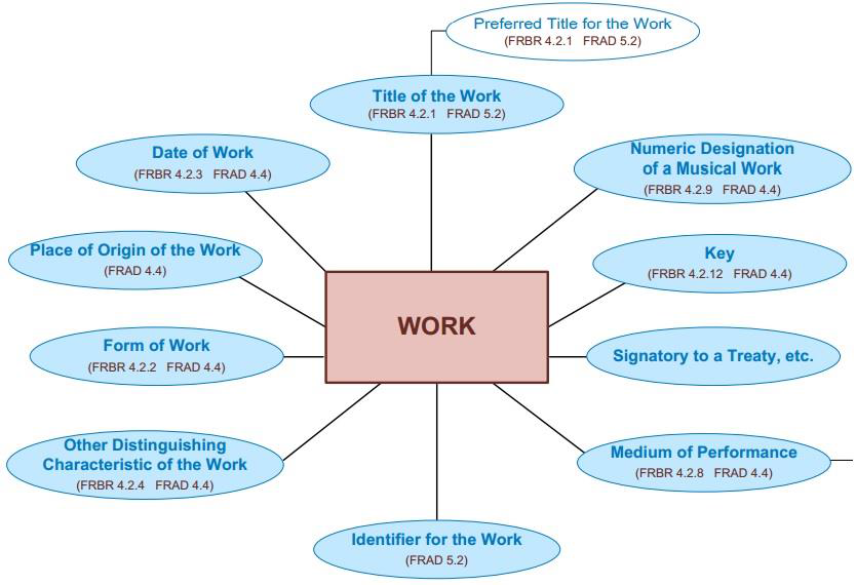
\includegraphics[width=0.75\textwidth]{./dados/figuras/exemplo_fig2.png}
\fonte{Disponível em \url{http://www.rdatoolkit.org/}.}
\end{figure}


%Inserir seu texto...
\lipsum[13-14]



\subsection{Seção terciária}

%Inserir seu texto...
\lipsum[15-17]
      % Referencial teórico
% PROCEDIMENTOS METODOLÓGICOS------------------------------------------------

\chapter{PROCEDIMENTOS METODOLÓGICOS}\label{metodologia}

%Inserir seu texto... (remova os comandos \lipsum[*], eles apenas inserem textos "defaul" de exemplo)
\lipsum[18-20]


  % Metodologia
% ANÁLISE DOS RESULTADOS-----------------------------------------------------

\chapter{ANÁLISE DOS RESULTADOS}\label{resultados}

Eitis mundus veius se porteirus \cite{AntonBivensDavis2007}.
A vidis is duris pra quienis is moles \cite{AntonRorres2012}.


%Inserir seu texto... (remova os comandos \lipsum[*], eles apenas inserem textos "defaul" de exemplo)
\lipsum[21-22]

%Quadro 1
\begin{quadro}[H]

\caption{Título do primeiro quadro}\label{quad1}
\centering
\begin{tabular}{|C{0.125\textwidth} |C{0.125\textwidth} |C{0.125\textwidth} |C{0.125\textwidth} |C{0.125\textwidth} |C{0.125\textwidth} |}  %<--- veja definição em pacotes.tex
 \hline
 & & & & & \tabularnewline
 \hline
 & & & & & \tabularnewline
 \hline
 & & & & & \tabularnewline
 \hline
 & & & & & \tabularnewline
 \hline
 & & & & & \tabularnewline
\hline

\hline
\end{tabular}
\fonte{Adaptado de \citen[p. 66]{BergmanEA2015}.}
\end{quadro}




\lipsum[23-28]




%Quadro 2
\begin{quadro}[H]

\caption{Título do segundo quadro}\label{quad2}
\centering
\begin{tabular}{|C{0.1\textwidth} |C{0.1\textwidth} |C{0.1\textwidth} |C{0.1\textwidth} |C{0.1\textwidth} |C{0.1\textwidth} |C{0.1\textwidth} |C{0.1\textwidth} |}  %<--- veja definição em pacotes.tex
 \hline
 & & & & & & & \tabularnewline
 \hline
 & & & & & & & \tabularnewline
 \hline
 & & & & & & & \tabularnewline
 \hline
 & & & & & & & \tabularnewline
 \hline
 & & & & & & & \tabularnewline
\hline

\hline
\end{tabular}
\fonte{\citen[p. 77]{AzevedoFernandes2015}.}
\end{quadro}


\lipsum[29-31]



%------------------ Tabela 1
\begin{table}[H]
\caption{Título da primeira tabela}\label{tab1}
\centering
\begin{tabular}{C{0.3\textwidth} C{0.3\textwidth} C{0.3\textwidth}}  %<--- veja definição em pacotes.tex
\hline
\textbf{Peso X} & \textbf{Estatura Y} & \textbf{Idade Z} \tabularnewline
\hline
35 & 128 & 13 \tabularnewline
38 & 140 & 13 \tabularnewline
45 & 140 & 14 \tabularnewline
52 & 150 & 15 \tabularnewline
\hline
\end{tabular}
\fonte{Elaborado pelo autor.}
\end{table}




\lipsum[32]




%------------------ Tabela 2
\begin{table}[H]
\caption{Título da segunda tabela}\label{tab2}
\centering
\begin{tabular}{C{0.3\textwidth} C{0.3\textwidth} C{0.3\textwidth}}  %<--- veja definição em pacotes.tex
\hline
\textbf{XXX} & \textbf{XXXXX} & \textbf{XXXX} \tabularnewline
\hline
10\% & 1 & 20 \tabularnewline
20\% & 2 & 30 \tabularnewline
30\% & 3 & 50 \tabularnewline
\hline
\end{tabular}
\fonte{Elaborado pelo autor.}
\end{table}


\lipsum[33]

As Equações~\ref{eq1} e \ref{eq2} são exemplos de uso do ambiente \textit{equation} para inserção de objetos matemáticos. Não se esqueça que é possível inserir objetos matemáticos no modo \textit{in-line}, por exemplo, $\displaystyle e=\sum _{{n=0}}^{{\infty }}{\frac  {1}{n!}}$.


%------------------ Equacão 1
\begin{equation}\label{eq1}
{\textrm{D}}_\textrm{B}(X,Y) &= N \left[\frac{\log|{\Sigma}_{X}|+\log|{\Sigma}_{Y}|}{2}-\log\left|\left(\frac{{\Sigma}_{X}^{-1}+{\Sigma}_{Y}^{-1}}{2}\right)^{-1}\right|\right]
\end{equation}


%------------------ Equacão 2
\begin{equation}\label{eq2}
F(\mathbf{x}) = \textrm{sgn} \left( \sum_{i=1}^{m} \alpha_i K(\mathbf{x},\mathbf{x}_{i}) - b \right)
\end{equation}

   % Resultados
% CONSIDERAÇÕES FINAIS-------------------------------------------------------

\chapter{CONSIDERAÇÕES FINAIS}\label{conclusoes}

%Inserir seu texto... (remova os comandos \lipsum[*], eles apenas inserem textos "defaul" de exemplo)
\lipsum[33-34]


    % Conclusão

\postextual
% INSERE ELEMENTOS PÓS-TEXTUAIS
% REFERÊNCIAS------------------------------------------------------------------

% Carrega o arquivo "base-referencias.bib" e extrai automaticamente as referências citadas
\renewcommand\bibname{REFERÊNCIAS}
\bibliography{./base-referencias}
\bibliographystyle{abntex2-alf} % Define o estilo ABNT para formatar a lista de referências
% OBSERVAÇÕES------------------------------------------------------------------
% Este arquivo não precisa ser alterado.
   % Referências
% APÊNDICES--------------------------------------------------------------------

%Ajustar para "APÊNDICE", caso possua um único apêndice
\addcontentsline{toc}{chapter}{APÊNDICES}


% Primeiro apêndice------------------------------------------------------------
% Edite para alterar o título deste apêndice
\chapter*{APÊNDICE A -- Título do apêndice}\label{apendiceA}


Texto em formato livre.




% Segundo apêndice------------------------------------------------------------
% Edite para alterar o título deste apêndice
\chapter*{APÊNDICE B -- Título do apêndice}\label{apendiceB}



Texto em formato livre.

     % Apêndice A, B, C, ...
% ANEXO------------------------------------------------------------------------

%Ajustar para "ANEXO", caso possua um único anexo
\addcontentsline{toc}{chapter}{ANEXOS}


% Primeiro anexo------------------------------------------------------------
% Edite para alterar o título deste anexo
\chapter*{ANEXO A -- Título do anexo}\label{apendiceA}


Texto em formato livre.




% Segundo anexo------------------------------------------------------------
% Edite para alterar o título deste anexo
\chapter*{ANEXO B -- Título do anexo}\label{apendiceB}



Texto em formato livre.        % Anexos A, B, C, ...

\end{document}